\documentclass[letterpaper,12pt]{article}
\usepackage[utf8]{inputenc}
\usepackage{fullpage}
\usepackage{courier}
\usepackage[margin=0.75in]{geometry}
\usepackage{listings}
\usepackage{color}
\usepackage{graphicx}
\usepackage[width=4in]{caption}
\usepackage{hyphenat}

% Format a sectionless paragraph
\newcommand*\unparagraph{
	\par
	\nopagebreak
	\vskip3.25ex plus1ex minus.2ex
	\noindent
}

% define extra colors
\definecolor{dkgreen}{rgb}{0,0.6,0}
\definecolor{purple}{RGB}{159,0,197}

% define the code listing format
\lstset{
	language=C++,
	basicstyle=\ttfamily,
	backgroundcolor=\color{white},
	showspaces=false,
	showstringspaces=false,
	frame=none,
	tabsize=3,
	keywordstyle=\color{purple},
	commentstyle=\color{dkgreen},
	stringstyle=\color{blue},
	escapeinside={\%*}{*)}
}

% efine the title/header
\title{\Large CS 1428\\Quiz 4 Sections L19 and L06} 
\author{Jared Wallace}
\date{}

\begin{document}

\maketitle

% code example here
\unparagraph{}
\begin{lstlisting}[basicstyle=\footnotesize\ttfamily]
int myFunction(int number, float &big)
{
	cout << big << " " << number;
	number = number * 10;
	big = number;
	return number;
}
\end{lstlisting}

\begin{enumerate}
	\item Which is the function prototype for the above function?
		\begin{enumerate}
			\item void myFunction(int, float);
			\item int myFunction(int, float);
			\item int myFunction(int, float\&);
			\item int MyFunction(int, float\&);
		\end{enumerate}
   \item For the following function call, what will \textbf{display} to the screen? \lstinline$myFunction(3, 2);$
		\begin{enumerate}
			\item 2  3
			\item 3  2
			\item 23  32
			\item 32  23
		\end{enumerate}
	\item What type of data will the function return for the above function call?
		\begin{enumerate}
			\item double
			\item float
			\item void (none)
			\item int
		\end{enumerate}

\newpage

   \item What is wrong with the following function definition? (two possible answers, pick the best/easiest one to implement)
		\begin{lstlisting}
void getInfo()
{
	cout << "Please enter your first name: ";
	cin >> name;
}
		\end{lstlisting}
		\begin{enumerate}
			\item There is a missing semicolon after getInfo()
			\item It should not be a void function
			\item The prompt is not courteous enough
			\item The function has no access to name, it should have been passed as a parameter
		\end{enumerate}
\end{enumerate}

\vspace{35mm}

% Comic at the bottom
\begin{figure}[ht!]
	\centering
	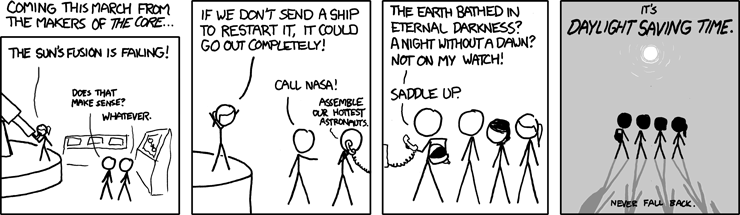
\includegraphics[width=6in]{the_sun.png}
	\caption*{}
\end{figure}

\end{document}
